\chapter{Signal with Memory - Random Processes}
\label{ch:part2}

\section{a. Autokorrelation}
I denne opgave skal vi se på forskellige tilfældigt gereret signaler og deres relation til hukommelse. Vi skal også stifte bekendskab med Markov modellen som vi vil gøre brug af i denne aflevering.\\
\subsection{Markov modellen}
Markov modellen er en måde, at lave en stokatsisk proces hvor tilstanden udelukkende bestemmes af den tidligere tilstand. Man kunne overføre methoden til den fysiske verden ved at udtrykke det som, jo højer sansynligheden er for at tilstanden skifter, jo højer er frekvensen fra modellen. Markov modellen har stor relation med hukommelse i en proces. Hvis sandsynligheden er 50$\%$ for at tilstanden skifter er det dermed et udtryk for at der ingen hukommelse er i processen da der lige stor sandsynlighed for et tilstands skifte, hvis sansynligheden er tættere på 1 eller 0 vil hukommelsen være større i processen. \\

 På figure \ref{fig:part2_1} er en Markov tilstands matrix hvori sansynligheden for tilstands skift er beskrevet:  

På figure \ref{fig:part2_2} er et Markov diagram som visuelt beskriver Markov matrixen:

 \begin{figure}[!h]
	\centering
	\subfloat[Markov matrix ]{%
		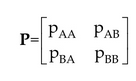
\includegraphics[width=0.2\textwidth]{resources/part2_markov_matrix}
		\label{fig:part2_1}}
	\subfloat[Markov diagram]{%
		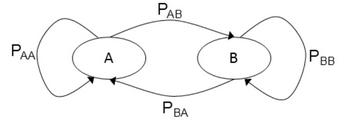
\includegraphics[width=0.4\textwidth]{resources/part2_markov_diagram}
		\label{fig:part2_2}}
	\caption{Markov model med tilstandsmatrix og tilhørende diagram}
	\label{fig:part2_markov}
\end{figure}
 

\subsection{Autokorrelation}
Autokorrelation af en tilfældig proces beskriver værdierne i den tilfældige proces til forskellige tidspunkter. Denne methode kan benyttes til at finde hukommelse i en proces. Vi vil se på hvordan autokorrelationen ser ud på en enkelt tilfældig proces og tilsvarende hvordan den arter sig ved gennemsnittet af mange gentaelser af processer.

Vi vil lave forsøget 3 slags signaler  

\begin{enumerate}
	\item Ensartet fordelt pseudotilfældige numre (rand i matlab)   figur \ref{fig:part2_3}
	\item Normalfordelt pseudotilfældige numre (randn i matlab)figur\ref {fig:part2_4}
	\item 1. ordens Markov model med to tilstande uden hukommelse. figur \ref{fig:part2_5}
	\item 1. ordens Markov model med to tilstande med hukommelse. figur \ref{fig:part2_6} 
\end{enumerate}

På begge figure, er den øverste illustration af selve rand/randn processen. Den midster illustration er af en enkelt realisering af det autokorrelateret signal og den nederste illustration auto korrelateringen  af 100 realisering.  
 \begin{figure}[!h]
	\centering
	\subfloat[ Ensartet fordelt pseudotilfældige numre]{%
		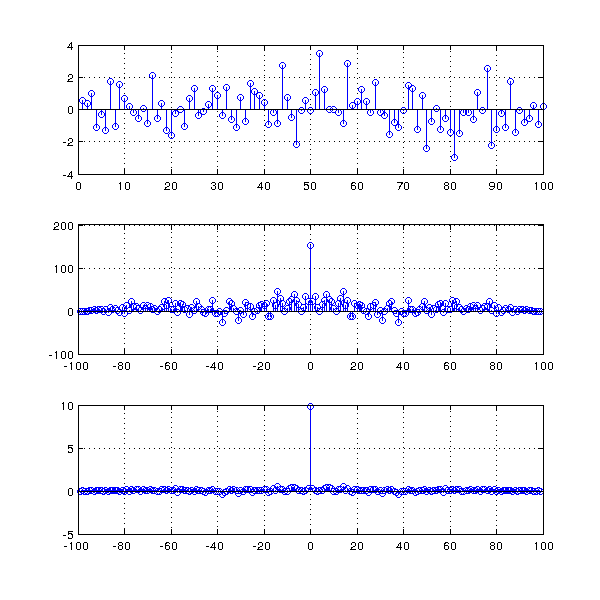
\includegraphics[width=0.6\textwidth]{resources/part2_rand}
		\label{fig:part2_3}}
	\subfloat[normalfordelt pseudotilfældige numre]{%
		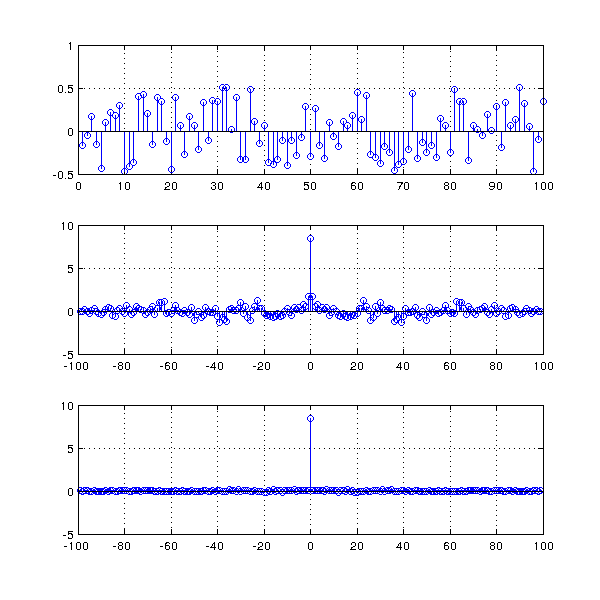
\includegraphics[width=0.6\textwidth]{resources/part2_randn}
		\label{fig:part2_4}}
	\caption{ Ensartet fordelt pseudotilfældige og normalfordelt pseudotilfældige numre med autokorrlation }
	\label{fig:part2_ran}
\end{figure}

 \begin{figure}[!h]
	\centering
	\subfloat[Markov model uden hukommelse]{%
		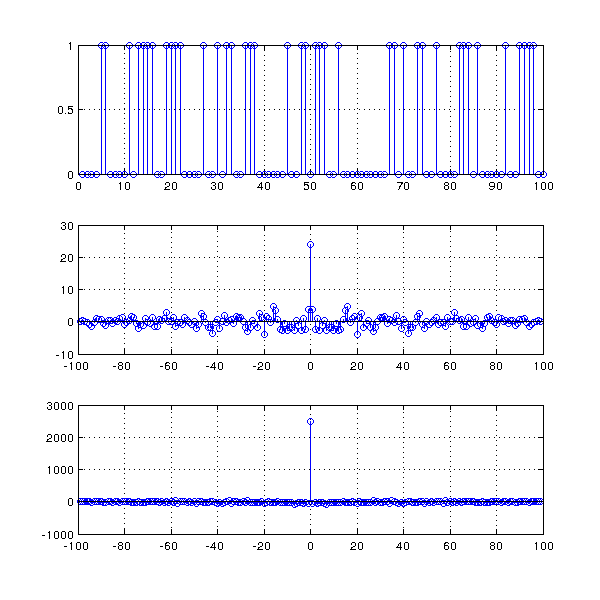
\includegraphics[width=0.55\textwidth]{resources/part2_markov_uden}
		\label{fig:part2_5}}
	\subfloat[Markov model med hukommelse]{%
		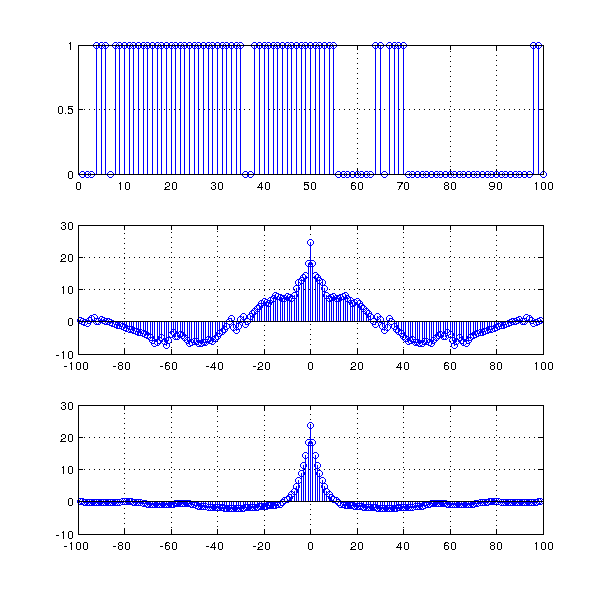
\includegraphics[width=0.55\textwidth]{resources/part2_markov_med}
		\label{fig:part2_6}}
	\caption{Markov model med og uden hukommelse }
	\label{fig:part2_markov}
\end{figure}
Således kan vi fastslå at hukommelsen i en proces kan analyseres ved hjælp af autokorrlation.

\section{b. Entropi }
Entropi er et mål i bit, som beskriver forudsiglighed af informationsindhold i en proces.

 \begin{figure}[!h]
	\centering
	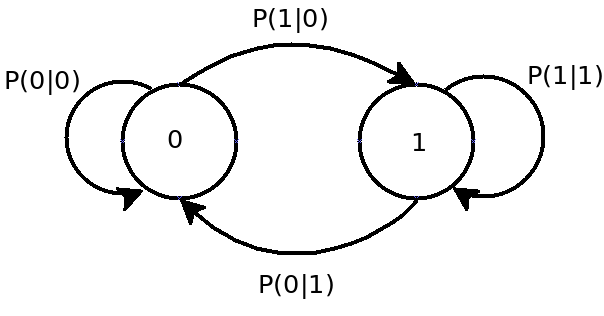
\includegraphics[width=0.6\textwidth]{resources/part2_entropi_diagram}
	\caption{Markov trasient diagram for entropi }
	\label{fig:part2_7}
\end{figure}
Og tilsvarende kan vi opstille en markov overgangs matrix:

\[ \left( \begin{array}{ccc}
P(0|0) & p(0|1)  \\
P(1|0) & P(1|1) \end{array} \right)\] 

Vi skal udfra viden om entropi, finde entropien for et system med og et uden hukommelse.\\
Vi finder entropien ved:
\begin{equation}
H(X) = P(0)H(X|0)+P(1)H(X|1)
\end{equation}
Hvor
\begin{equation}
H(X|0)=p(0|0)log_2 \bigg(\frac{1}{P(0|0)}\bigg)+P(1|0)log_2\bigg(\frac{1}{P(1|0)}\bigg)
\end{equation}
\begin{equation}
H(X|1)=p(0|1)log_2 \bigg(\frac{1}{P(0|1)}\bigg)+P(1|1)log_2\bigg(\frac{1}{P(1|1)}\bigg)
\end{equation}

P(0) og P(1) finder vi ved at løse disse to ligninger med de to ubekendte:

\begin{equation}
P(0) = P(0|0)P(0)+P(1|0)P(1)
\end{equation}

\begin{equation}
P(1)=P(1|0)P(0)+P(0|1)P(1)
\end{equation}

Hvor
\begin{equation}
P(0)+P(1)=1
\end{equation}

Vi laver en proces med hukommelse og finder entropien for denne tilfældige proces:\\ vi opstiller en Markov overførings matrix for procesen:

\[ \left( \begin{array}{ccc}
P(0|0) = 0.92 & p(1|0) = 0.08   \\
P(0|1) = 0.12  & P(1|1) = 0.88  \end{array} \right)\] 

Vi udregner $P(X|0)$ og $P(X|1)$:

\begin{equation}
H(X|0)=0.92log_2 \bigg(\frac{1}{0.92}\bigg)+0.08log_2\bigg(\frac{1}{0.08}\bigg) = 0.402
\end{equation}
\begin{equation}
H(X|1)=0.12log_2 \bigg(\frac{1}{0.12}\bigg)+0.88log_2\bigg(\frac{1}{0.88}\bigg) = 0.529
\end{equation}

Derefter finder vi $P(0)$ og $P(1)$:

\begin{equation}
P(0) = 0.6 \\,\\P(1) = 0.4
\end{equation}

Vi bruger ligning 2.1 til at finde $H(X)$:

 \begin{equation}
H(X) = 0.6\cdot 0.402+0.4 \cdot 0.529 = 0.453 bit/symbol
\end{equation} 



\begin{equation}
H(x)_{hukommelse}<H(x)_{ingen hukommelse}
\end{equation}



\section{c.}

Wiener-Khinchin Teorem hedder, at energi tæthedsspektrumet af en tilfældig proces er fouier transformationen af autokorrlationens funktionen. Det vil med andre ord betyde at vi kan lave et energy spektrugram ved at lave en fouier transformation på den autokorrlaieret proces.
 
Autokorrelationsfunktionen for en realisering af processen er en stokastisk signal i sig selv - mens autokorrelation af processen er et helt deterministisk signal.





